\{\% set num = 15\%\} \{\% set titre = ``Algorithmes gloutons''\%\} \{\%
set theme = ``algorithmique'' \%\} \{\% set niveau = ``premiere''\%\}

\{\{ titre\_chapitre(num,titre,theme,niveau)\}\}

\hypertarget{activituxe9s}{%
\subsection{Activités}\label{activituxe9s}}

\{\{ titre\_activite(``Introduction'',{[}{]},0) \}\}

!!! note ``Problème d'optimisation : Le voyageur'' \textbf{Enoncé du
problème :}\\
Un voyageur souhaite visiter plusieurs villes de France, dans n'importe
quel ordre, mais en minimisant la distance parcourue.

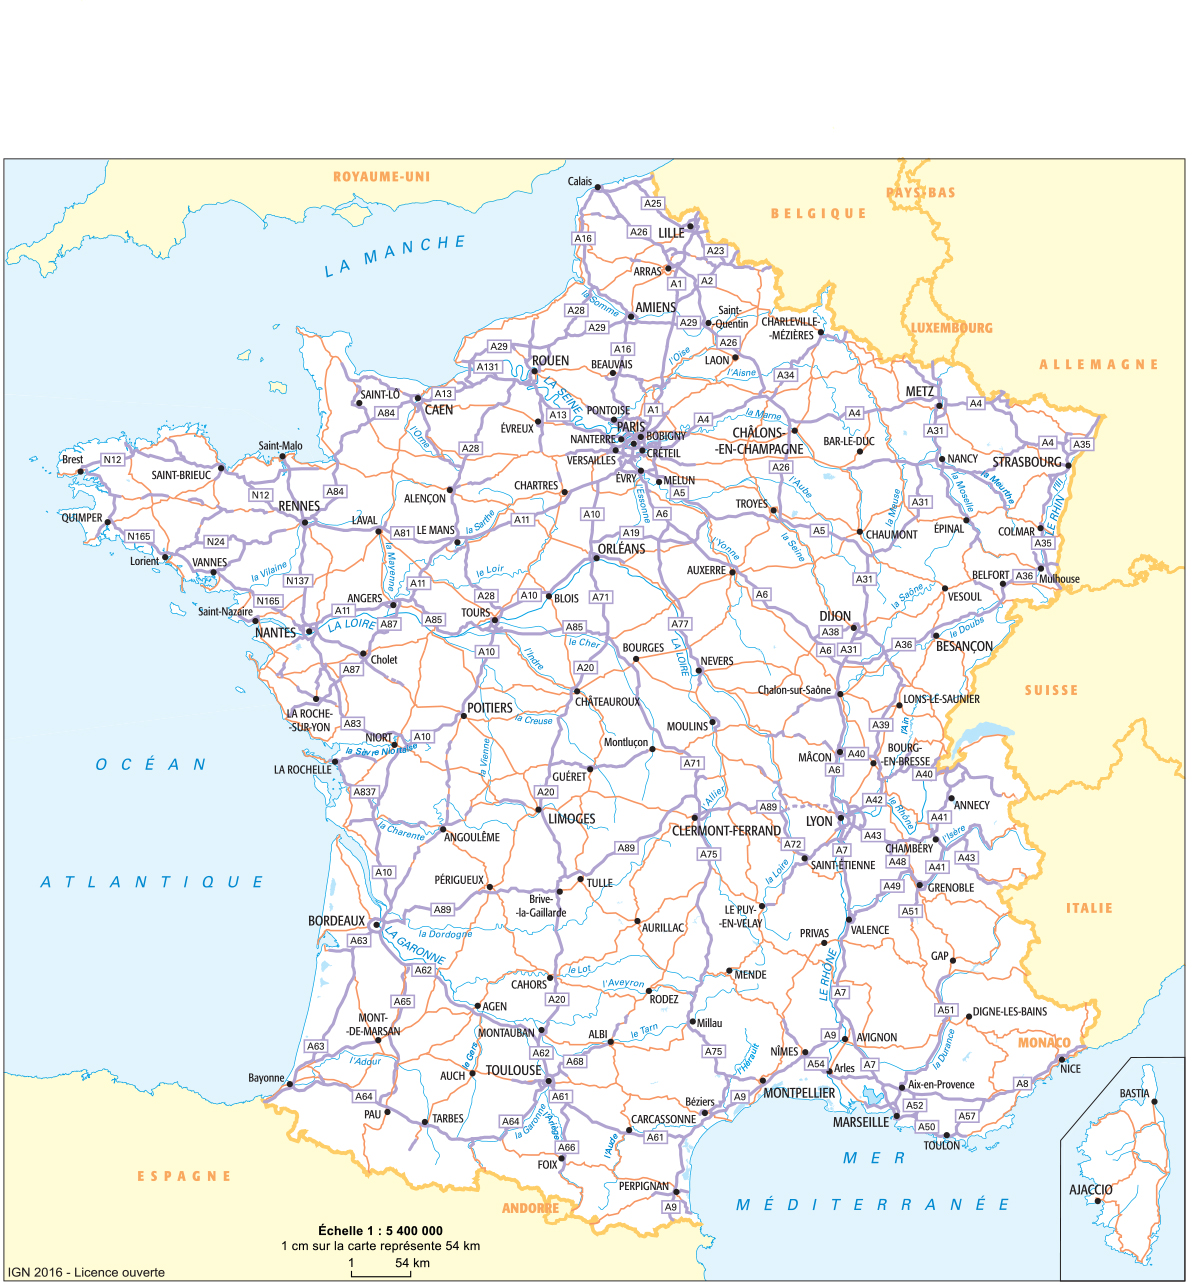
\includegraphics{data/carte_route.jpg}\{:.center width=75\%\}

Le tableau suivant donne les distances routières kilométriques entre
plusieurs villes de France :

\begin{longtable}[]{@{}ccccccccc@{}}
\toprule
& \textbf{Clermont-Ferrand} & \textbf{La Rochelle} & \textbf{Lille} &
\textbf{Limoges} & \textbf{Lyon} & \textbf{Marseille} & \textbf{Nantes}
& \textbf{Paris}\tabularnewline
\midrule
\endhead
\textbf{La Rochelle} & 462 & & & & & & &\tabularnewline
\textbf{Lille} & 622 & 688 & & & & & &\tabularnewline
\textbf{Limoges} & 173 & 222 & 608 & & & & &\tabularnewline
\textbf{Lyon} & 165 & 614 & 681 & 385 & & & &\tabularnewline
\textbf{Marseille} & 413 & 823 & 1001 & 593 & 314 & & &\tabularnewline
\textbf{Nantes} & 534 & 137 & 600 & 320 & 655 & 986 & &\tabularnewline
\textbf{Paris} & 423 & 472 & 225 & 392 & 466 & 775 & 385
&\tabularnewline
\textbf{Toulouse} & 377 & 421 & 894 & 290 & 467 & 404 & 585 &
678\tabularnewline
\bottomrule
\end{longtable}

\textbf{Question 1 :}

\begin{itemize}
\tightlist
\item
  Départ et arrivée à Clermont-Ferrand,\\
\item
  Villes à visiter : Limoges, Lyon, Paris et Toulouse.
\end{itemize}

\textbf{Q1.a} Combien de ``chemin'' possible ?

\textbf{Q1.b} Déterminer tous les chemins possibles ainsi que le
kilométrage totale.

\textbf{Q1.c} Répondre au problème: quel est le trajet optimal ?

Le problème se ramène à trouver un ordre de visite des quatre villes
pour lequel la somme des distance données par ce tableau est aussi
petite que possible.\\
Une manière simple d'aborder le problème consiste à énumérer tous les
cas possibles et calculer la distance correspondante pour chacun des
cas.

\textbf{Question 2 :}\\
Calculer le nombre de trajets possibles si le voyageur décide de visiter
toutes les villes du tableau.

??? tip Cette technique (répertorier tous les cas de figure et faire une
étude exhaustive) n'est pas possible à grande échelle.\\
Déterminer le nombre d'itinéraires possibles :

\begin{verbatim}
* 8 villes (hors ville de départ) on a : $\dfrac{8 \times 7 \times 6 \times 5 \times 4 \times 3 \times 2 \times 1}{2}= 20160$ itinéraires possibles.  
* 10 villes (hors ville de départ), nombre d'itinéraires à tester : $\dfrac{10 \times 9 \times 8 \times 7 \cdots \times 2 \times, 1}{2}=$ 1 714 400  
* 13 villes (hors ville de départ), nombre d'itinéraires à tester : $\dfrac{13 \times 12 \cdots \times 2 \times, 1}{2}=$ 3 113 510 400  
* 20 villes (hors ville de départ), nombre de parcours à tester :  $\dfrac{20 \times 19 \times 18 \times 17 \cdots \times 2 \times, 1}{2}=$ 1 216 451 004 088 320 000   
> Face à de tels problèmes d'optimisation impossible à explorer exhaustivement, il peut être utile de connaître des algorithmes donnant rapidement une réponse qui, sans être nécessairement optimale, resterait bonne.
\end{verbatim}

\hypertarget{synthuxe8se}{%
\subsubsection{Synthèse}\label{synthuxe8se}}

Nous avons vu que la force brute ne permet pas de résoudre (en un temps
raisonnable) le problème du voyageur de commerce lorsqu'on augmente le
nombre de villes.

Maintenant que vous avez manipulé ce problème et vu à quel point il est
complexe à résoudre, nous allons voir comment faire autrement.

!!! jeretiens ``A retenir :'' - Les \textbf{algorithmes gloutons}
(greedy algorithms) constituent une alternative beaucoup plus simple à
programmer, mais dont le résultat n'est pas toujours optimal (sauf dans
certaines situations dites canoniques) - L'approche gloutonne consiste à
construire une solution complète par une succession de choix locaux
donnant systématiquement la meilleure solution partielle.

\begin{verbatim}
Pour résumer, on peut employer un algorithme glouton lorsque :  

- une solution complète peut être construite en passant par une succession de solutions partielles,  
- chaque solution partielle est établie en faisant un choix local à partir de la solution partielle précédente,  
- on dispose d’une fonction permettant d’évaluer la qualité de chaque solution partielle.  

_Les choix ne sont jamais remis en cause : une fois faits, on ne revient pas dessus. Cela constitue une différence essentielle avec la programmation dynamique qui au lieu de se focaliser sur un seul sous-problème, explore les solutions de tous les sous-problèmes pour les combiner finalement de manière optimale._
\end{verbatim}

Les \textbf{algorithmes gloutons} sont utilisés pour répondre à des
\textbf{\emph{problèmes d'optimisation}}, c'est-à-dire des problèmes
algorithmiques dans lesquels l'objectif est de trouver une solution " la
meilleure possible " selon un critère, parmi un ensemble de solutions
également valides mais potentiellement moins avantageuses.

Le contexte général d'un tel problème d'optimisation est donc le suivant
: b

\begin{itemize}
\tightlist
\item
  on considère un problème possédant un très grand nombre de solutions\\
\item
  on dispose d'une fonction mathématique évaluant la qualité de chaque
  solution\\
\item
  on cherche une solution qui soit bonne, voire meilleure.
\end{itemize}

Les algorithmes gloutons s'appliquent lorsque de plus : * la recherche
d'une solution peut se ramener à une succession de choix qui produisent
et précisent petit à petit une solution partielle * on dispose d'une
fonction mathématique évaluant la qualité de chaque solution partielle
(dont on attend qu'elle soit cohérente avec la fonction d'évaluation des
solutions complètes).

!!! exo ``Retour à l'activité'' Répondre à la question de l'activité en
appliquant cet algorithme.

\{\{ titre\_activite(``Mise en oeuvre avec Python'',{[}{]},) \}\}

\{\{capytale(``6774-1470050'')\}\}

\{\{ titre\_activite(``Le problème du sac à dos'',{[}{]},) \}\}

Dans un jeu vidéo, le héros dispose d'un sac à dos lui permettant de
porter les objets collectés au fil du jeu, avec une capacité maximale de
10 kg.\\
Le héros souhaite maximiser la valeur en pièces d'or des objets contenus
dans le sac à dos, qui varie de 3 à 30 pièces d'or selon l'objet.\\
L'objectif est d'aider le héros à effectuer cette optimisation.

\begin{longtable}[]{@{}cccccccc@{}}
\toprule
Objet & Antidote & Baguette magique & Cape d'invisibilité & Diadème &
Epée & Horloge & Miroir\tabularnewline
\midrule
\endhead
Numéro objet & 1 & 2 & 3 & 4 & 5 & 6 & 7\tabularnewline
Valeur (pièces d'or) & 3 & 5 & 12 & 15 & 9 & 10 & 12\tabularnewline
Masse (kg) & 0.5 & 1 & 1 & 5 & 6 & 5 & 3\tabularnewline
Valeur massique & & & & & & &\tabularnewline
\bottomrule
\end{longtable}

!!! question ``Q1'' Classer ces objets par valeur décroissante et donner
la solution de l'algorithme glouton avec ce critère de classement.

!!! question ``Q2''\\
Même question avec un classement par poids croissant.

!!! question ``Q3''\\
Même question avec un classement par valeur/poids (valeur massique)
croissant.

!!! question ``Q4''\\
A-t-on obtenu la solution optimale ?

\textbf{Activité Capytale :} \{\{capytale(``cd2e-1484556'')\}\}

\{\{ titre\_activite(``Rendu de monnaie'',{[}{]},) \}\}

!!! note ``Présentation du problème'' Un achat dit en espèces se traduit
par un échange de pièces et de billets. Pour simplifier, considérons que
les pièces désignent indifféremment les véritables pièces ou les
billets.\\
Supposons qu'un achat induise un rendu de monnaie 49 euros.\\
Quelles pièces peuvent être rendues ? La réponse n'est pas unique :

\begin{verbatim}
- Quatre pièces de 10 euros, 1 pièce de 5euros et deux pièces de 2e uros conviennent.  
- Mais quarante-neuf pièces de 1 euros conviennent également !  

Si la question est de rendre la monnaie avec un minimum de pièces, la réponse reste simple : c’est la première solution proposée.  
Toutefois, comment parvient-on à un tel résultat ? Quels choix ont été faits qui optimisent le nombre de pièces rendus ?  
\end{verbatim}

Le problème est de rendre la monnaie en un minimum de pièces.\\
La solution dépend évidemment du système de monnaie utilisé.\\
Considérons le système monétaire européen simplifié où les pièces
prennent les valeurs 500, 200, 100, 50, 20, 10, 5, 2 , 1 euros. Rendre
49 euros avec un minimum de pièces est un problème d'optimisation. En
pratique, sans s'en rendre compte généralement, tout individu met en
œuvre un algorithme glouton.\\
Il choisit d'abord la plus grandeur valeur de monnaie, parmi 1, 2, 5,
10, contenue dans 49 euros. En l'occurrence, quatre fois un pièce de 10
euros. La somme de 9 euros restant à rendre, il choisit une pièce de 5
euros, puis deux pièces de 2 euros.\\
Mais cette stratégie gagnante pour la somme de 49 euros l'est-elle pour
n'importe quelle somme à rendre ?

!!! info ``Application du paradigme glouton''

!!!exo ``Exercice 1'' 1. On considère le système monétaire européen
systeme = {[}1, 2, 5, 10, 20, 50, 100, 200, 500{]}. Quelle est la
solution gloutonne pour un rendu de monnaie de 34 euros?\\
de 47 euros ?

\begin{verbatim}
2. On considèrele système monétaire systeme = [1, 3, 6, 12, 24, 30]. Quelle est la solution gloutonne pour un rendu de monnaie de 49 euros ? Est-elle optimale ? 
\end{verbatim}

!!! note ``Remarque :'' Un système monétaire pour lequel l'algorithme de
rendu de monnaie glouton donne toujours un nombre minimal de pièces est
dit canonique. Il existe des algorithmes permettant de déterminer si un
système monétaire est canonique.

\hypertarget{activituxe9-sur-capytale}{%
\subsubsection{Activité sur Capytale}\label{activituxe9-sur-capytale}}

\textbf{Activité Capytale :} \{\{capytale(``5726-1484553'')\}\}
